\section{Scelte implementative}
\label{cap:implementation-choices}

\subsection{Codice templatizzato}

\subsection{Rappresentazione del grafo}

Le due possibilità standard per rappresentare un grafo sono 
\begin{itemize}
	\item \textbf{Matrici di adiacenza}
	\item \textbf{Liste di adiacenza}
\end{itemize}

In questa implementazione abbiamo scelto di utilizzare una lista di adiacenza affiancata da una struttura dati aggiuntiva unordered\_set per migliorare i tempi di alcune operazioni fondamentali. Il relativo diagramma di classe è possibile ri-trovarlo nella figura~\ref{fig:AdjListGraph Class} dove vengono riportati gli attributi e i metodi offerti dalla classe.

\begin{figure}[h]
	\caption{Diagramma di classe per AdjListGraph}
	\centering
	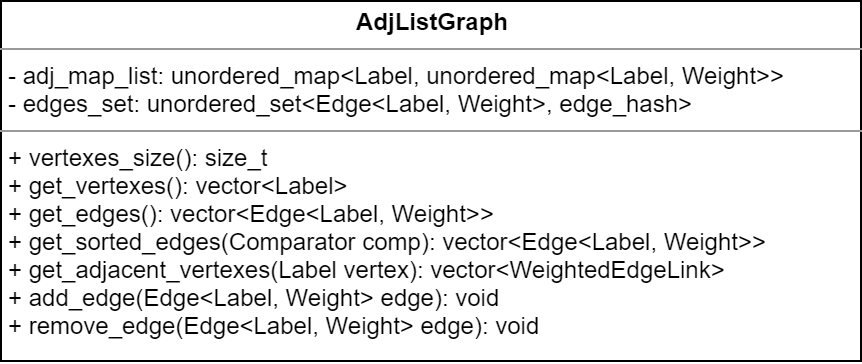
\includegraphics[width=0.7\textwidth]{./images/AdjListGrapClassDiagram.png}
	\label{fig:AdjListGraph Class}
\end{figure}

Nonostante la lista di adiacenza sarebbe già sufficiente per salvare tutte le informazioni necessarie alla rappresentazione di un grafo, in alcune operazioni risulta essere lenta. L'esempio di operazione che ci ha spinto ad inserire una nuova struttura dati (unordered\_set in questo caso) è il metodo per ritornare tutti gli archi di un grafo in quanto tale metodo se implementato avendo a disposizione la sola lista di adiacenza prevederebbe in maniera semplice la scansione dell'intera lista di adiacenza, con l'inserimento degli archi che si ritrovano in ogni vertice. Tale semplice implementazione porterebbe alla creazione di un vettore in cui se sussiste un arco tra un vertice 2 e un vertice 3, il vettore conterebbe sia l'arco 2 $\rightarrow$ 3 e 3 $\rightarrow$ 2 per costruzione della lista di adiacenza. \\

Le cose si complicano maggiormente se si restringe la richiesta di non restituire gli archi doppi come abbiamo già osservato. A tale proposito si potrebbe ricercare l'eventuale presenza di tali archi doppi ed eliminarli di conseguenza, ma il tutto richiederebbe maggiori operazioni e dunque un maggior tempo di esecuzione.\\

Per tali ragioni è stato deciso di affiancare alla lista di adiacenza, un'apposita struttura dati che permettesse di tenere traccia degli archi e di avere tempi di esecuzione costanti per le operazioni di aggiunta, rimozione e ricerca. Così facendo è possibile garantire che l'operazione di restituzione degli archi singoli di un grafo abbia tempo O(m) se si richiede di restituire un vettore, o addirittura O(1) se si richiede la restituzione di un puntatore a tale struttura.
E' stato scelto dunque di utilizzare come struttura dati da affiancare unordered\_set perchè oltre ad avere le caratteristiche richieste, se appositamente configurata permette di garantire l'assenza di archi doppi, compresi quelli visti nell'esempio precedente (ossia 2 $\rightarrow$ 3 e 3 $\rightarrow$ 2). Per fare ciò è stato dunque opportunamente configurato l'operatore di uguaglianza e la funzione di hash, in  modo che archi equivalenti abbiamo la stessa funzione di hash e siano riconosciuti come uguali, evitando così l'inserimento di un arco doppio visto che che unordered\_set non prevede elementi doppi al suo interno.\\

Una rappresentazione astratta di tale struttura è possibile visualizzarla nella figura~\ref{fig:edges_set}, dove è possibile notare che se viene richiesto l'inserimento di un arco 3 $\rightarrow$ 2 ove già presente un arco 2 $\rightarrow$ 3 questo non viene inserito da unordered\_set.\\

\begin{figure}[h]
	\caption{Visualizzazione astratta di edges\_set}
	\centering
	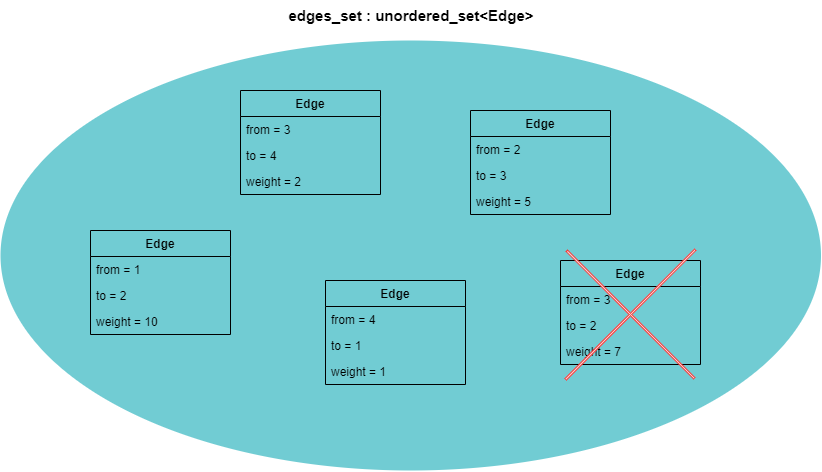
\includegraphics[width=0.7\textwidth]{./images/edges_setAbstract.png}
	\label{fig:edges_set}
\end{figure}

L'ultimo problema non ancora affrontato rigurda la possibilità di inserire un arco doppio tra due nodi uguali (come richiesto da problema), con la differenza che questi 2 archi hanno un peso diverso. Siccome la nostra implementazione non prevede la presenza di tali archi doppi, la funzione add\_eddge() si occupa di verificare l'eventuale presenza di un arco già inserito e di conseguenza i relativi pesi, per andare a modificare il peso qualora il peso del nuovo arco sia inferiore al peso dell'arco precedentemente già inserito. Per fare questo ad ogni aggiunta di un nuovo arco si va a verificare nella lista di adiacenza l'esistenza di un arco per quei due vertici:
\begin{itemize}
	\item \textbf{se l'arco era già stato aggiunto:} si confrontano i due pesi e si aggiorna il peso dell'arco solo nell'eventualità in cui il nuovo peso sia inferiore a quello già presente nella lista di adiacenza. Dopodichè se c'è stato un aggiornamento si aggiorna anche il relativo unordered\_set, eliminando l'arco precendente e si riaggiunge l'arco con il nuovo peso. 
	\item \textbf{se l'arco non era già stato inserito:} si inserisce l'arco sia nella lista di adiacenza che nell'unordered\_set.
\end{itemize}

Tutte le operazioni di aggiunta, per come sono implementati unordered\_set e unordered\_map in C++ hanno tempo costante e dunque l'operazione di aggiunta richiede tempo costante.


\subsubsection{Strutture Dati}

\subsubsection{Binary Heap}

\iffalse
The class that implements a Binary Heap data structure
can be instantiated as a MinHeap or a MaxHeap at compile-time. \\

We spared the \complexityN{} time required to build the heap at the beginning of Prim's algorithm because the \textit{std::vector} we use to initialize the list already respects the MinHeap property: the key related to the first element is 0, and every other key is $+\infty$. \\
\fi

\subsubsection{Priority Queue}

\subsubsection{Disjoint Set}

\subsection{Algoritmi}

\subsubsection {Costruzione del Grafo}
In questa parte si va a leggere il file di input per poi darlo in pasto alla funzione di costruzione della rappresentazione del grafo come spiegato nella sezione precedente.......

\subsubsection{Prim con Binary Heap}

\subsubsection{Kruskal Naive}
L'algoritmo Kruskal Naive è stato implementato a partire dallo pseudo codice visto in classe. A partire da questo ci si è subito accorti che una delle peculiarità di tale algoritmo e la necessità di verificare ad ogni iterazione la presenza di un ciclo a seguito dell'inserimento dell'arco di peso minimo. Per ottenere tale funzionalità abbiamo deciso di modificare DFS in maniera da rilevare la presenza di un ciclo in un grafo. Per fare questo è stato creata la classe DFSCycleDetection, che è possibile ritrovare nella cartella "Shared", che data la rappresentazione del grafo e richiamando l'apposito metodo has\_cycle() è in grado di rilevare la presenza di un ciclo all'interno di esso usando per l'appunto una visita in profondità.\\

E' stato pertanto necessario modificare la visita in profondità nel seguente modo:
\begin{itemize}
	\item non è necessario avere una label per ogni arco che etichetti quell'arco come "DISCOVERY EDGE" o "BACK EDGE"
	\item quando un arco verrebbe eticchettato come "BACK EDGE" nello pseudo codice visto in classe possiamo affermare che nel grafo è presente un ciclo. Non è necessario riscostruire tutto il ciclo come visto in classe.
	\item al posto di tener traccia di ogni arco se è stato visitato o meno attraverso un attributo per ogni arco, è stato deciso di creare un set di archi già visitati dove l'inseriemento e la ricerca avviene in tempo costante.
	\item per essere sicuri di non prendere in considerazione il vertice da cui viene lanciata ricorsivamente la dfs (ossia per non ritrovare il nodo da cui siamo venuti) è stata passata alla ricorsione il vertice padre, in modo che quando si scansiona la lista di adiacenza del vertice in considerazione non si consideri il vertice padre, simulando così il comportamento della funzione "opposite(v,e)" nel pseudo codice.
\end{itemize}


Per risolvere il problema di piu di un eventuale componenente connessa nel grafo, vengono sempre scansionati tutti i nodi non ancora visitati attraverso un ciclo for su tutti i nodi come visto in classe.

Sono state poi aggiunte delle migliorie come la verifica di 3 nodi e l'arrivo a m-1 archi

Tale algoritmo risulta avere complessita O(mn)
Una volta creata la rappresentazione per il grafo,



\subsubsection{Kruskal con Disjoint Set}
